% !TEX TS-program = pdflatex
% !TEX encoding = UTF-8 Unicode
% !TEX ROOT = main.tex
\section{Gebäudeplan Kirchhoff-Institut für Physik (KIP)}
\begin{figure}[H]
\centering
\begin{subfigure}[h]{0.8\textwidth}
\centering
\includegraphics[width=\linewidth]{raumplan/eg}
\vspace*{5mm}
\end{subfigure}
\begin{subfigure}[h]{0.8\textwidth}
\centering
\includegraphics[width=\linewidth]{raumplan/og2}
\end{subfigure}
\end{figure}

\begin{figure}[H]
\centering
\begin{subfigure}[h]{0.8\textwidth}
\centering
\includegraphics[width=\linewidth]{raumplan/og1}
\vspace*{5mm}
\end{subfigure}
\begin{subfigure}[h]{0.8\textwidth}
\centering
\includegraphics[width=\linewidth]{raumplan/og3}
\vspace*{2mm}
\end{subfigure}
\begin{subfigure}[h]{0.8\textwidth}
\centering
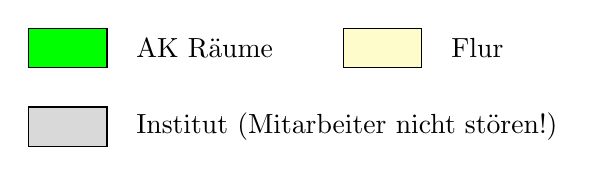
\begin{tikzpicture}	
\draw[fill=green] (0,0) rectangle (1,0.5);
\node[right] at (1.25,0.25) {AK Räume};
\draw[fill=yellow!20] (4,0) rectangle (5,0.5);
\node[right] at (5.25,0.25) {Flur};
\draw[fill=gray!30] (0,-1) rectangle (1,-0.5);
\node[right] at (1.25,-0.75) {Institut (Mitarbeiter nicht stören!)};
\end{tikzpicture}
\end{subfigure}
\end{figure}
